\chapter{Visual odometry}
\label{ch:vo}

Visual odometry (VO) estimates the camera's motion from its images,
frame after frame, without trying to build a globally consistent map.
It is to vision what wheel odometry is to the wheels: dead reckoning,
locally accurate and globally drifting. This chapter assembles the
pieces of Part~II into a complete stereo VO. Its new ingredient is the
pose of a camera from 3D points it sees (the Perspective-$n$-Point
problem); the rest is engineering: keyframes, tracking, map renewal. We
run the result on a simulated garden mown in rows, and measure how and
why it drifts. That drift, and its causes, set the agenda of Part~III.

\section{Pose from known points}

\begin{definition}{Perspective-$n$-Point}{pnp}
Given $n$ world points $\vect{X}_i$ and their normalised images
$\vect{x}_i$, find $T_{cw}=(R,\vect{t})$ with $\tilde{\vect{x}}_i\sim
R\vect{X}_i+\vect{t}$ for all $i$.
\end{definition}

The pose has six degrees of freedom and each point gives two equations,
so three points should suffice. They do, up to a finite ambiguity; with
more points we can afford a linear method.

\begin{proposition}{Linear PnP}{pnpdlt}
Write $P=[R\ \vect{t}]$ with rows $\vect{p}^{k\mathsf T}$, $k=1,2,3$,
and $\tilde{\vect{X}}=(\vect{X},1)$. Each correspondence gives the two
linear equations
\[
\vect{p}^{1\mathsf T}\tilde{\vect{X}}-u\,\vect{p}^{3\mathsf T}
\tilde{\vect{X}}=0,\qquad
\vect{p}^{2\mathsf T}\tilde{\vect{X}}-v\,\vect{p}^{3\mathsf T}
\tilde{\vect{X}}=0
\]
in the twelve entries of $P$. With $n\ge6$ points in general position
the solution is unique up to a scale $\lambda$, and $R$, $\vect{t}$ are
recovered from $\hat P=\lambda P$ by $\lambda=\sqrt[3]{\det\hat P_{1:3}}$
and $R=\mathrm{nearest}(\hat P_{1:3}/\lambda)$, $\vect{t}=\hat
P_4/\lambda$. If all the points lie on a plane, the system has a null
space of dimension at least four and the method fails.
\end{proposition}

\begin{proof}
$\tilde{\vect{x}}\sim P\tilde{\vect{X}}$ means $u=\vect{p}^{1\mathsf T}
\tilde{\vect{X}}/\vect{p}^{3\mathsf T}\tilde{\vect{X}}$ and similarly for
$v$; clearing the denominator gives the equations, as in
\cref{prop:dlt}. $P$ has eleven degrees of freedom up to scale, so six
points (twelve equations) are needed in general. Since $\det(\lambda R)=
\lambda^3$, the real cube root of $\det\hat P_{1:3}$ recovers $\lambda$
with its sign; with noise $\hat P_{1:3}/\lambda$ is only close to a
rotation, and \cref{lem:nearestrot} projects it. For the degeneracy,
choose world coordinates in which the plane is $Z=0$: then the entries
$p_{13},p_{23},p_{33}$ multiply $Z_i=0$ in every equation, so the three
corresponding unit vectors are in the null space, in addition to the
true solution.
\end{proof}

A lawn is exactly this degenerate case, and it would be with any world
frame, since the degeneracy is a property of the point set. The planar
problem is a homography problem instead: for points on the plane $Z=0$,
$\tilde{\vect{x}}\sim[\vect{r}_1\ \vect{r}_2\ \vect{t}](X,Y,1)\T$, which
is the extrinsic step of Zhang's calibration (Exercise~\ref{ex:7plane}).
Minimal solvers do not suffer from it.

\begin{proposition}{The P3P equations}{p3p}
Let $\vect{b}_i=\tilde{\vect{x}}_i/\norm{\tilde{\vect{x}}_i}$ be the unit
bearings of three points, $c_{ij}=\vect{b}_i\T\vect{b}_j$, and
$d_{ij}=\norm{\vect{X}_i-\vect{X}_j}$. The unknown distances
$s_i>0$ from the optical centre to the points satisfy
\begin{equation}\label{eq:p3p}
s_i^2+s_j^2-2c_{ij}\,s_is_j=d_{ij}^2,\qquad (i,j)\in\{(1,2),(2,3),
(1,3)\}.
\end{equation}
Eliminating two unknowns leads to a polynomial of degree four in the
third, so there are at most four solutions. Each gives the points in
the camera frame, $\vect{q}_i=s_i\vect{b}_i$, and the pose follows from
the three pairs $(\vect{X}_i,\vect{q}_i)$ by \cref{prop:umeyama}.
\end{proposition}

\begin{proof}
In the camera frame the centre is the origin and the $i$-th point is
$s_i\vect{b}_i$. The distance between two points is preserved by the
rigid motion, so $d_{ij}^2=\norm{s_i\vect{b}_i-s_j\vect{b}_j}^2$, which
expands to \eqref{eq:p3p}: the law of cosines in the triangle formed by
the centre and the two points. The elimination to a quartic is classical
(Grunert, 1841); modern solvers (Kneip et al., 2011; Persson and
Nordberg's Lambda Twist, 2018) obtain the same roots more stably.
\end{proof}

\begin{inwords}
Three bearings and three known distances define a rigid tetrahedron with
the camera at its apex; there can be up to four ways to fit it. A fourth
point decides between them, which is why our RANSAC samples four points:
three for the solver, one to choose. The notebook shows a typical case,
with one solution 18\,m away from the truth that reprojects the fourth
point 84 pixels wrong.
\end{inwords}

\section{Motion-only bundle adjustment}

\begin{definition}{Motion-only bundle adjustment}{mba}
With map points $\vect{X}_j$ held fixed, refine the camera pose by
minimising the robust reprojection error
\[
T_{wc}^\star=\arg\min_{T_{wc}}\ \tfrac12\sum_j\rho\Bigl(\bigl\|\z_j-
h(T_{wc},\vect{X}_j)\bigr\|^2_{\Sigma}\Bigr),
\]
where $h$ is the projection of \cref{prop:projjac} (monocular, $\z_j\in
\R^2$) or the rectified stereo projection of \cref{def:stereo}
($\z_j=(u_l,v,u_r)$), and $\rho$ a robust kernel.
\end{definition}

It is the problem of Chapter~\ref{ch:nls} with the Jacobians of
Chapter~\ref{ch:cameras}: $\partial h/\partial\bxi=(\partial h/\partial
\vect{q})\,[\,-I\ \ \hatop{\vect{q}}\,]$, with $\vect{q}=T_{wc}^{-1}
\vect{X}_j$. The stereo version adds the right-image column, which makes
the depth of each point part of the measurement. The pipeline is always
the same: a minimal solver in RANSAC for a robust start, then this
refinement on all points with a redescending kernel. Each step matters
(\cref{fig:pnp}, left; notebook, section~3): with 35\,\% outliers, the
RANSAC pose is 4\,cm off; least-squares refinement from it ends 5\,m
away, dragged by the outliers RANSAC rejected; the Cauchy refinement
ends at 9\,mm.

\begin{figure}[ht]
\centering
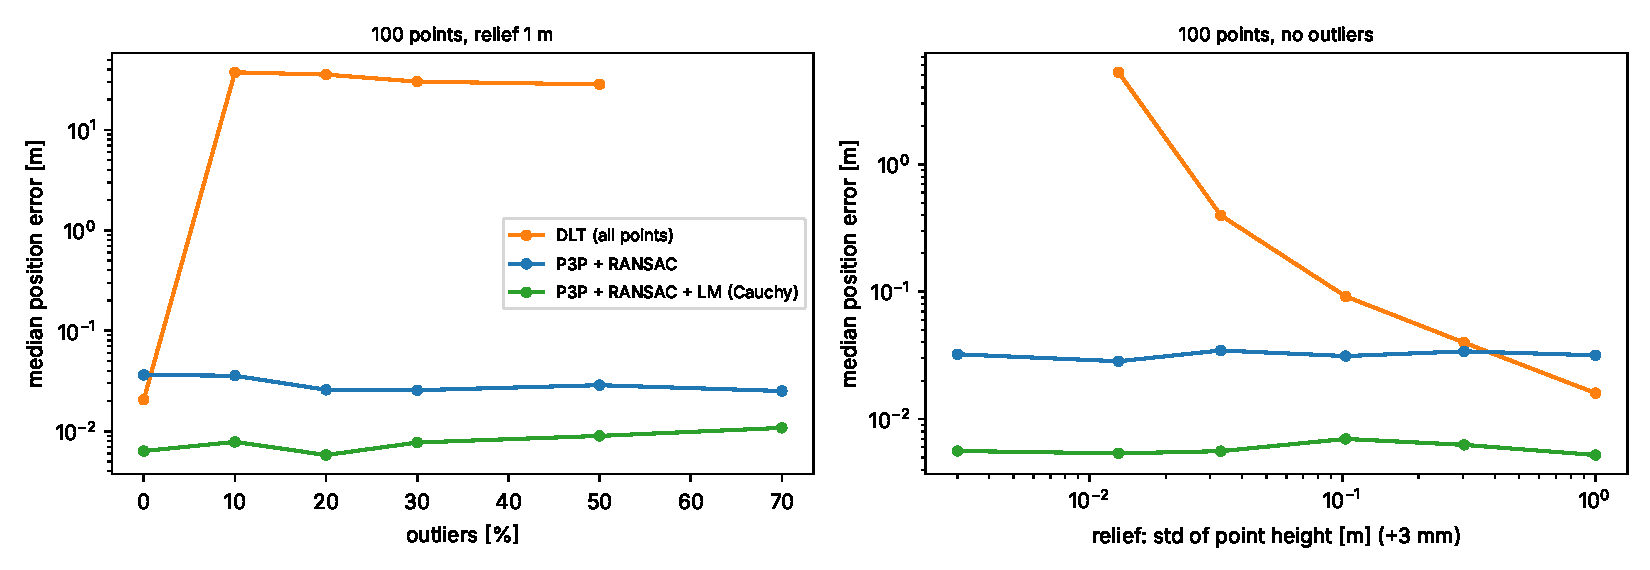
\includegraphics[width=\linewidth]{figures/ch07_pnp.pdf}
\caption{Camera position from 100 known points, 0.5\,px noise (median
of 20 trials). Left: with outliers; the linear PnP breaks at the first
one, P3P in RANSAC does not, and the robust refinement divides its error
by five. Right: as the scene flattens, the linear PnP degrades and fails
on a plane; P3P is unaffected.}
\label{fig:pnp}
\end{figure}

\section{A stereo visual odometry}

\paragraph{The pipeline.} Our stereo VO (\code{vslam.vo.StereoVO}) is
deliberately minimal:
\begin{enumerate}[nosep]
\item At a \emph{keyframe}, triangulate every tracked feature from its
  stereo measurement (\cref{prop:disparity}) and store the point, in
  world coordinates, under its track identifier: the local map.
\item At every new frame, collect the tracked features whose identifiers
  are in the map and localise the camera against those points: P3P in
  RANSAC, then motion-only bundle adjustment with a Cauchy kernel on the
  stereo measurements.
\item Create a new keyframe when fewer than half of the map points are
  still tracked as inliers, or when the camera has moved more than 1\,m
  or turned more than $15^\circ$ since the keyframe.
\end{enumerate}
In a real system the tracks come from the front-end of
Chapter~\ref{ch:features}: Lucas--Kanade between consecutive left
images, the right image matched along the epipolar line (a row, after
rectification), new corners detected where the image has few. Here they
come from \code{vslam.sim}, which simulates that front-end's output
geometrically: noisy stereo measurements of the landmarks of a garden,
tracks that end at random --- after 9 frames in median, sooner on grass
--- and a few wrong measurements (2\,\% on structure, 10\,\% on grass).
A landmark that is seen again after its track ended gets a new
identifier: the VO cannot recognise places, it can only follow tracks.

\begin{figure}[ht]
\centering
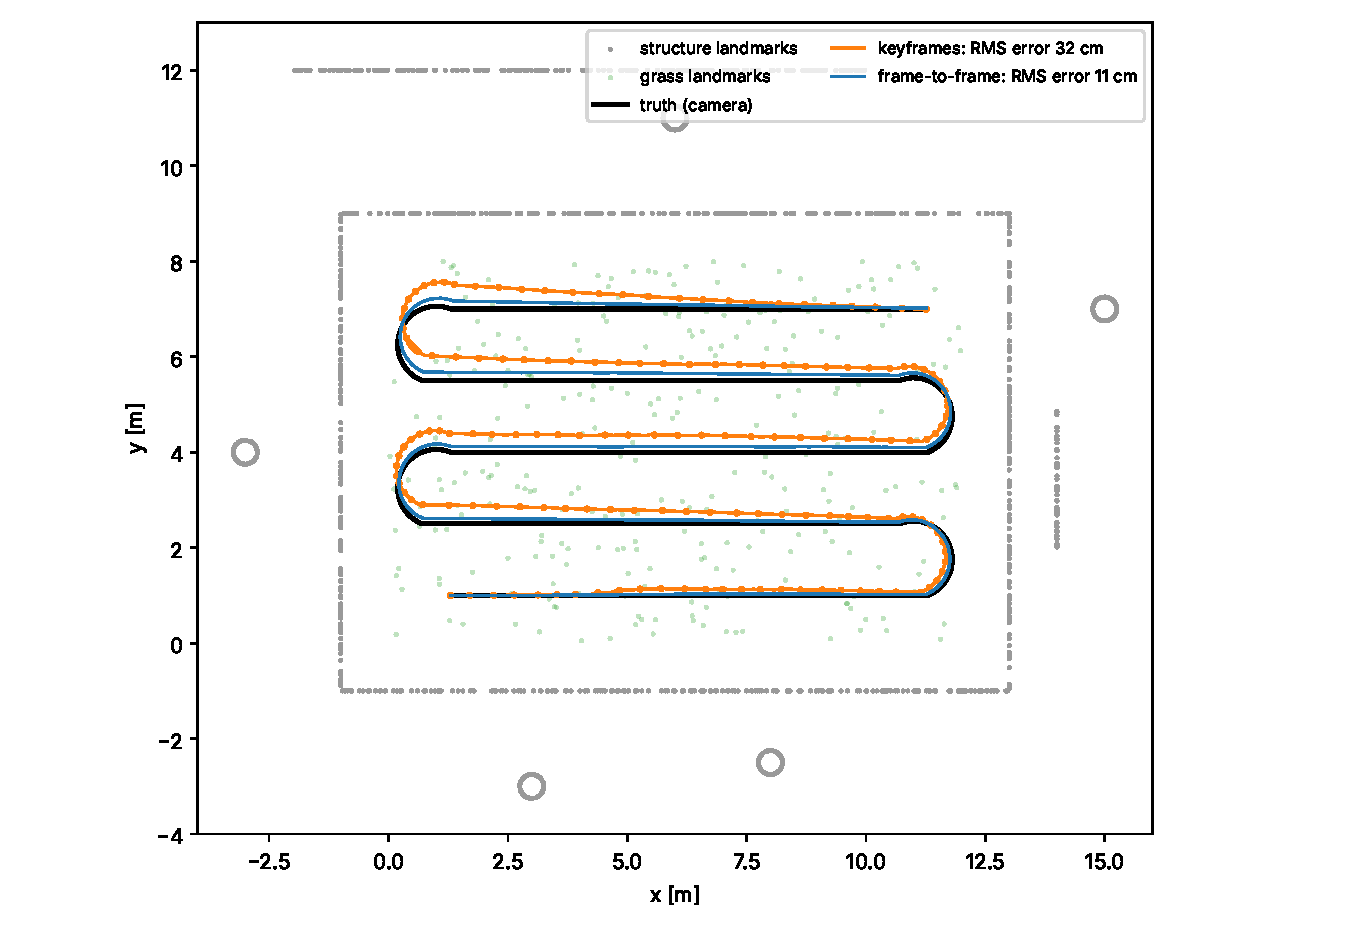
\includegraphics[width=0.85\linewidth]{figures/ch07_vo.pdf}
\caption{The simulated garden (grey: fence, house wall, shed and tree
trunks; green: points on the lawn) and 60\,m of mowing in five rows at
5\,cm per frame. Camera 0.8\,m high, pitched down $15^\circ$, stereo
baseline 12\,cm, 0.5\,px noise. Black: truth; orange: keyframe VO, with
its keyframes as dots; blue: frame-to-frame VO (a keyframe at every
frame).}
\label{fig:vo}
\end{figure}

\paragraph{What happens.} Both variants follow the rows without a single
tracking failure, and both drift (\cref{fig:vo}): after 60\,m the RMS
position error is 32\,cm for the keyframe VO and 11\,cm for the
frame-to-frame one. That the keyframe version does \emph{worse} deserves
an explanation, because it contradicts the usual advice. Its map is
triangulated once, from a 12\,cm baseline, and then used unchanged for
up to a metre of motion. By \cref{prop:disparity} a point 5\,m away has
a depth error of 20\,cm, and every frame localised against it inherits a
bias that grows with the distance from the keyframe and is the same for
all those frames. The frame-to-frame version re-triangulates at every
frame; its map errors are drawn afresh each time and partly cancel.

The usual advice is not wrong, though. Let the mower stand still, with
long-lived tracks (\cref{fig:drift}, right): the frame-to-frame VO adds
a little noise at every frame and drifts by 4\,cm in 20\,s without
moving, whereas the keyframe VO keeps its map and stays put. A mower
stops often --- to turn, to empty its basket, to let someone pass. The
two experiments together say what the next chapter will do: keep
keyframes, but stop treating their map points as exact. Refine them with
every frame that sees them. That is local bundle adjustment.

\begin{proposition}{How heading errors accumulate}{driftlaw}
A vehicle moves in the plane by steps of length $L$. Before each step its
heading receives an independent error $\epsilon_i\sim\Normal(0,\sigma^2)
$, so that after $i$ steps the heading error is $\varphi_i=\sum_{j\le i}
\epsilon_j$. To first order in the $\varphi_i$, the lateral position
error after $n$ steps has standard deviation
\[
\sigma_y(n)=L\,\sigma\sqrt{\frac{n(n+1)(2n+1)}6}\ \approx\ \frac{L\,
\sigma}{\sqrt3}\,n^{3/2} .
\]
By contrast, independent errors of standard deviation $\sigma_L$ on the
step lengths alone give a longitudinal error growing like $\sigma_L
\sqrt n$.
\end{proposition}

\begin{proof}
The lateral displacement is $y_n=\sum_{i=1}^nL\sin\varphi_i\approx L
\sum_{i=1}^n\varphi_i=L\sum_{i=1}^n\sum_{j=1}^i\epsilon_j=L\sum_{j=1}^n
(n-j+1)\epsilon_j$. The $\epsilon_j$ are independent, so
$\operatorname{Var}y_n=L^2\sigma^2\sum_{j=1}^n(n-j+1)^2=L^2\sigma^2
\sum_{m=1}^nm^2$, and $\sum_{m=1}^nm^2=n(n+1)(2n+1)/6$. The longitudinal
statement is the variance of a sum of $n$ independent errors.
\end{proof}

\begin{inwords}
Errors in position add up like a random walk, growing as the square
root of the distance. Errors in heading are worse: each one turns every
later step, and their effect grows as the distance to the power $3/2$ ---
the banana of Chapter~\ref{ch:rigid} in another guise. The VO of
\cref{fig:drift} (left) grows roughly linearly, between the two laws,
because its heading is not a pure random walk: distant landmarks (the
house, the trees) observe the orientation directly
(\cref{prop:projjac}: rotation moves every pixel, whatever its depth).
This is why VO drift is commonly quoted as a percentage of the distance
travelled, here about 1\,\%.
\end{inwords}

\begin{figure}[ht]
\centering
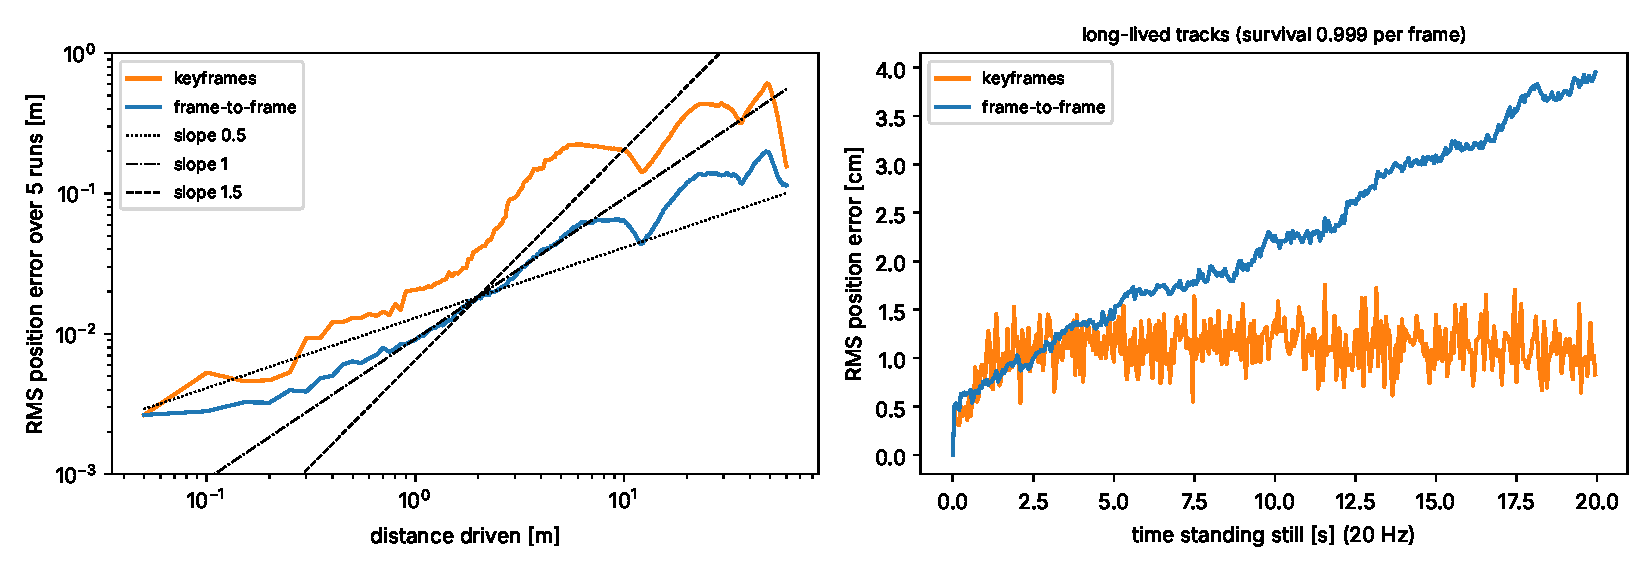
\includegraphics[width=\linewidth]{figures/ch07_drift.pdf}
\caption{Left: RMS position error over 5 runs versus distance driven,
with reference power laws. Right: position error while the mower
stands still for 20\,s, with tracks that last (survival 0.999 per
frame): the keyframe VO stays at its noise level, the frame-to-frame VO
drifts.}
\label{fig:drift}
\end{figure}

\section{Measuring drift}

An estimated trajectory and the true one are expressed in frames that
need not agree: the VO fixes its gauge with its first pose
(Chapter~\ref{ch:slam}), a motion-capture system or RTK-GNSS uses its
own. Comparing them therefore starts with an alignment.

\begin{proposition}{Optimal alignment}{umeyama}
For points $\vect{e}_i$ (estimate) and $\vect{g}_i$ (truth), $i=1,\dots,
n$, with centroids $\bar{\vect{e}},\bar{\vect{g}}$ and centred versions
$\vect{E}_i$, $\vect{G}_i$, the similarity minimising $\sum_i\norm{
\vect{g}_i-(sR\vect{e}_i+\vect{t})}^2$ is
\[
R=\mathrm{nearest}\Bigl(C\Bigr),\ \ C=\sum_i\vect{G}_i\vect{E}_i\T,\qquad
s=\frac{\tr(R\T C)}{\sum_i\norm{\vect{E}_i}^2},\qquad
\vect{t}=\bar{\vect{g}}-sR\bar{\vect{e}},
\]
where $\mathrm{nearest}$ is the projection of \cref{lem:nearestrot}. For
a rigid alignment, set $s=1$.
\end{proposition}

\begin{proof}
For fixed $(s,R)$ the cost is a convex quadratic in $\vect{t}$, whose
gradient vanishes at $\vect{t}=\bar{\vect{g}}-sR\bar{\vect{e}}$.
Substituting, the cost becomes $\sum_i\norm{\vect{G}_i-sR\vect{E}_i}^2=
\sum_i\norm{\vect{G}_i}^2-2s\tr(R\T C)+s^2\sum_i\norm{\vect{E}_i}^2$,
using $\sum_i\vect{G}_i\T R\vect{E}_i=\tr(R\T C)$ and $\norm{R
\vect{E}_i}=\norm{\vect{E}_i}$. For any $s>0$ it is minimised by the
rotation maximising $\tr(R\T C)$, which is the nearest rotation to $C$
(proof of \cref{lem:nearestrot}). Then it is a quadratic in $s$,
minimised at the value given.
\end{proof}

\begin{definition}{ATE and RPE}{atrpe}
The \emph{absolute trajectory error} is the RMS of $\norm{\vect{g}_i-(s
R\vect{e}_i+\vect{t})}$ after the alignment of \cref{prop:umeyama}
($s=1$ for stereo or inertial systems, free for monocular ones). The
\emph{relative pose error} over a distance $\Delta$ is, for every pair of
poses $(i,j)$ separated by $\Delta$ metres of travel, the error
$\bigl(T^{\mathrm{gt}\,-1}_iT^{\mathrm{gt}}_j\bigr)^{-1}\bigl(T^{-1}_i
T_j\bigr)$, summarised by its translation (often as a percentage of
$\Delta$) and its rotation.
\end{definition}

ATE measures global consistency, the quantity that matters for a map;
RPE measures local accuracy and is insensitive to where the drift
happened. For our keyframe VO on the full run: 35\,cm RMS error without
alignment, 13\,cm ATE after alignment, and an RPE of 1.8\,\% over 1\,m
and 0.9\,\% over 20\,m (notebook, section 7).

\begin{mower}
One per cent of drift sounds small. At a 0.6\,m cutting width the mower
drives about 170\,m per 100\,m$^2$ of lawn; a 1\,000\,m$^2$ garden is
1.7\,km of driving and, at 1\,\%, some 17\,m of accumulated error by
the end --- dozens of rows. VO alone cannot keep the stripes straight.
Three things will fix it, and they are the rest of the course:
\begin{itemize}[nosep]
\item \emph{local bundle adjustment} (Chapter~8) to stop treating map
  points as exact and to make keyframes pay off;
\item \emph{loop closure} (Chapter~10): the mower passes the same fence
  and the same tree at every row, and recognising them removes the
  accumulated error;
\item \emph{fusion} (Part~IV): the IMU fixes roll and pitch and slows the
  heading drift, the wheels constrain short motions, and RTK-GNSS anchors
  everything when the sky is open.
\end{itemize}
Meanwhile, two lessons hold for the mower right away: localise on
structure, not on grass (the simulation drops grass tracks quickly, and
a real lawn is worse); and keep keyframes, because the mower stops.
\end{mower}

\begin{practice}[\code{vslam/pnp.py}, \code{vslam/vo.py},
  \code{vslam/sim.py}, \code{vslam/metrics.py}, \code{examples/ch07\_vo.py},
  \code{notebooks/ch07\_vo.ipynb}]
\begin{center}
\begin{tabular}{@{}ll@{}}
\toprule
Code & Formula\\
\midrule
\code{pnp.pnp\_dlt} & \cref{prop:pnpdlt}\\
\code{pnp.p3p}, \code{pnp.pnp\_ransac} & \cref{prop:p3p} (OpenCV
  solver), RANSAC\\
\code{pnp.MonoPoseProblem}, \code{StereoPoseProblem} & \cref{def:mba},
  vectorised\\
\code{vo.StereoVO} & the pipeline of Section 7.3\\
\code{sim.garden}, \code{boustrophedon}, \code{GardenSim} & the
  simulated garden\\
\code{metrics.align}, \code{ate}, \code{rpe} & \cref{prop:umeyama},
  \cref{def:atrpe}\\
\bottomrule
\end{tabular}
\end{center}
The tests check exact linear PnP and its rank deficiency on a plane,
that P3P contains the truth and works on a plane, robust PnP with 40\,\%
outliers, the vectorised pose Jacobians against finite differences, the
similarity alignment, a zero RPE for identical trajectories, the
continuity of the mowing pattern, exact stereo measurements in the
noise-free simulator, and the VO on a short run (exact without noise,
below 5\,\% of the distance with noise). The notebook adds the four P3P
solutions, the three refinement strategies, a camera view of the
simulated garden, the drift law against Monte Carlo, and ATE versus RPE.
\end{practice}

\section*{Further reading and C++ pointers}
\addcontentsline{toc}{section}{Further reading and C++ pointers}

D.~Scaramuzza and F.~Fraundorfer, ``Visual odometry'', parts I and II,
\emph{IEEE Robotics and Automation Magazine}, 2011--2012 (the tutorial);
D.~Nist\'er, O.~Naroditsky and J.~Bergen, ``Visual odometry'', CVPR
2004; V.~Lepetit, F.~Moreno-Noguer and P.~Fua, ``EPnP'', IJCV 2009;
L.~Kneip, D.~Scaramuzza and R.~Siegwart, ``A novel parametrization of
the perspective-three-point problem'', CVPR 2011; B.~K.~P.~Horn,
``Closed-form solution of absolute orientation using unit quaternions'',
JOSA 1987, and Umeyama (1991); J.~Sturm et al.\ (TUM RGB-D, 2012) for
ATE and RPE. In C++: OpenCV's \code{solvePnPRansac} (with
\code{SOLVEPNP\_AP3P}, \code{SOLVEPNP\_EPNP}, \code{SOLVEPNP\_SQPNP});
the trackers of ORB-SLAM3 and VINS-Fusion; the \code{evo} package for
evaluation.

\FloatBarrier
\section*{Exercises}
\addcontentsline{toc}{section}{Exercises}

\begin{enumerate}[label=\textbf{7.\arabic*},ref=7.\arabic*]
\item\label{ex:7plane} \emph{PnP on the lawn.} For points on the ground
  plane $Z=0$, show that $\tilde{\vect{x}}\sim H(X,Y,1)\T$ with
  $H\sim[\vect{r}_1\ \vect{r}_2\ \vect{t}]$, and explain how to recover
  the pose from four or more such points.
\item\label{ex:7gauge} Show that the ATE with rigid alignment does not
  change if the whole estimated trajectory is moved by a rigid motion.
  Why is this the right property?
\item\label{ex:7drift} A VO has a heading error of $0.005^\circ$ per 5\,cm
  step and nothing else. Using \cref{prop:driftlaw}, how large is the
  lateral error after 100\,m?
\item\label{ex:7stereo} In motion-only bundle adjustment, compare the
  information a single point gives about the camera's motion along its
  line of sight with a monocular and with a stereo measurement.
\end{enumerate}

\subsection*{Solutions}

\textbf{7.1.} With $Z=0$, $R\vect{X}+\vect{t}=X\vect{r}_1+Y\vect{r}_2+
\vect{t}=[\vect{r}_1\ \vect{r}_2\ \vect{t}](X,Y,1)\T$. Estimate $H$ from
four or more points by the DLT (in normalised coordinates, so $K=I$),
then proceed as in \code{calib.zhang\_extrinsics}: $\lambda=1/\norm{
\vect{h}_1}$, $\vect{r}_i=\lambda\vect{h}_i$, $\vect{t}=\lambda\vect{h}_3
$ with the sign giving positive depths, $\vect{r}_3=\vect{r}_1\times
\vect{r}_2$, and project onto $\SO3$.

\textbf{7.2.} Replacing $\vect{e}_i$ by $Q\vect{e}_i+\vect{c}$ replaces
the optimal $(R,\vect{t})$ by $(RQ\T,\vect{t}-RQ\T\vect{c})$, which gives
the same aligned points $R\vect{e}_i+\vect{t}$, hence the same errors.
The estimate's world frame is a gauge choice (\cref{prop:gauge}); a
metric must not reward or punish it.

\textbf{7.3.} $\sigma=0.005^\circ=8.73\times10^{-5}$\,rad, $L=0.05$\,m,
$n=2000$: $\sigma_y=0.05\times8.73\times10^{-5}\times\sqrt{2000\cdot2001
\cdot4001/6}\approx0.23$\,m. A heading error far below what any sensor
reports per step still costs a quarter of a metre over 100\,m.

\textbf{7.4.} With a monocular measurement, moving the camera along the
line of sight of a point does not move its image (the point stays on
the optical ray), so that point gives no information about this motion;
it only comes from other points through the geometry. A stereo
measurement includes the disparity $f_xb/Z$, which changes with $Z$:
each point constrains the motion along its own line of sight, with a
standard deviation $\sigma_Z=Z^2\sigma_\delta/(f_xb)$ by
\cref{prop:disparity}, good for near points and poor for far ones.
